\chapter{Plasma confinement}\label{sec:confinement}\thispagestyle{fancy}
%%
%%%%%%%%%% SECTION %%%%%%%%%% {{{1 Transport
\section{Transport}\label{sec:confinement:transport}
%%
%Lawson stated a criterion for any device to achieve fusion \cite{wesson}:
%\begin{align*}
	%n \tau_E T & > 5 \cdot 10^{-21} m^{-3} s\ keV
%\end{align*}
%%
The transport of energy and particle are governed by the conservation laws \cite{heatDiff,fable2006}
\begin{align}
	\dsdt{W_j} + \frac{1}{V'} \dsd{}{\rho} \left( V' q_j \right) & = S_j                                      & j = i,e \label{eq:confinement:transport:heat:heatDiff}\\
	\frac{1}{V'} \dsdt{} \left( V' n_e \right) + \frac{1}{V'} \dsd{}{\rho} \left( V' \Gamma_n \right) & = S_n           \label{eq:confinement:transport:particle:particleDiff}
\end{align}
where $W_j = \frac{3}{2} \intdd{V} n_j T_j$ with $j = e,i$, $S_j$ and $S_n$ denote respectively the heat and particle sources and sinks, $q_j$ and $\Gamma_n$ the heat and particle fluxes and $V' = \dsds{V}{\rho}$. The particle sources are mainly the gas injected, but also some interactions with the walls, thus it is localized at the edge of the plasma.

The heat sources are different whether we talk about the ions or the electrons. In the Tokamak \`a Configuration Variable (TCV), the electron heat sources are the ohmic heating and the electron cyclotron heating (ECH). There are no external ion heat source. Thus at TCV the electron temperature is higher than the ion temperature. Since this machine has dominant electron heating, the equipartition of energy (due to collisions) yields a source for the ions and a sink for the electrons. The heat sources are defined by \cite{heatDiff}
\begin{align*}
	S_e & = P_{\textrm{ohm}} + P_{\textrm{ECH}} - n_e \nu_{ei} ( T_e - T_i ) - P_{\textrm{rad}}\\
	S_i & = n_e \nu_{ei} ( T_e - T_i ) - P_{\textrm{rad}}
\end{align*}

The fluxes are given by the general equation \cite{wesson}
\begin{align*}
	\begin{pmatrix}
		\Gamma_n\\
		q_e\\
		q_i
	\end{pmatrix} & = - \mat{A}
	\begin{pmatrix}
		\nabla n_e\\
		\nabla T_e\\
		\nabla T_i
	\end{pmatrix}
\end{align*}
where the diagonal elements of $\mat{A}$ are the diffusion coefficients, $D_n$, $n_e \chi_e$ and $n_e \chi_i$. We usually assume that the heat fluxes depend mainly on the gradient of their species' temperature, which yields that the low-diagonal part of $\mat{A}$ is null, and so is $A_{23}$. We thus can write the heat fluxes as
\begin{align}
	q_j & = n_j \chi_j \nabla T_j   & j & = i, e             \label{eq:confinement:transport:heat:heatFlux}
\end{align}
	
On the other side, the particle flux may be somehow more complex thus much more difficult to compute, taking into account those crossed contributions. A simpler way to write it is
\begin{align}
	\Gamma_n & = - D_n \nabla n_e + V_n n_e \label{eq:confinement:transport:particle:particleFlux}
\end{align}
where $V_n$ is the pinch velocity and the convection term $V_n n_e$ could be seen as the contributions from the off-diagonal terms \cite{wesson}.

From a two-fluid model, we can compute the relation for the three diffusion coefficients \cite{freidberg}
\begin{align}\label{eq:confinement:transport:chis}
	D_n    & \sim \frac{\rho_{L,e}^2}{\bar{\tau}_{ei}} &
	\chi_i & \sim \frac{\rho_{L,i}^2}{\bar{\tau}_{ii}} &
	\chi_e & \sim \frac{\rho_{L,e}^2}{\bar{\tau}_{ee}}
\end{align}
where $\bar{\tau}_{ii}$ and $\bar{\tau}_{ee}$ are the mean time between collisions respectively for ions and for electrons, $\bar{\tau}_{ei}$ is the momentum exchange collision mean time and $\rho_{L,k}$ is the Larmor radius of species $k$.
%%
%for every physical quantity $Q$, where $D$ is the diffusivity and $S$ contains the sources and sinks. But this model does not provide the diffusion coefficients. To close the set of equations, one has to find them. The particle diffusion coefficient is deduced from the reduction of the model but the thermal diffusivities are still missing. Finding them can be done through a random walk model \cite{freidberg}. We thus find that $D = ( \Delta l )^2 / \tau$. After some computation, we can find that \cite{freidberg}
		
This is valid for the classical transport. Toroidal geometry implies other effects. This is the neoclassical transport theory. In this theory, we decompose the vector quantities into a parallel component (scalar) along the magnetic field, and a perpendicular component (vectorial) which is the other part. For instance, the velocity becomes $\vec{v} = v_{\Par} \vec{b} + \vec{v}_{\perp}$. We do not need to redo the whole computation to find the new diffusion coefficient. From simple calculations arise correction factors to the classical coefficients \cite{freidberg}, which we will not expand here.
%\begin{align*}
	%D_n^{(NC)}    & = 2.2  q^2 \left( \frac{R_0}{r} \right)^{\nicefrac{3}{2}} D_n^{(CL)}   \\
	%\chi_i^{(NC)} & = 0.68 q^2 \left( \frac{R_0}{r} \right)^{\nicefrac{3}{2}} \chi_i^{(CL)}\\
	%\chi_e^{(NC)} & = 0.89 q^2 \left( \frac{R_0}{r} \right)^{\nicefrac{3}{2}} \chi_e^{(CL)}
%\end{align*}

Neoclassical theory also predicts a very interesting phenomenon that is the bootstrap current \cite{freidberg}. In a magnetic tore, the outside of the tore has a lower magnetic field than the inside, because the amplitude is inversely proportional to the major radius. We respectively speak of \emph{low-field} and \emph{high-field side} of the tokamak. Moreover, the total magnetic field is helical, meaning the particles will have elliptic poloidal paths. Thus they may be trapped in the low-field side if they do not have enough parallel velocity to overcome the magnetic barrier. The bootstrap current arises from this through subtle transport phenomena \cite{freidberg}. It flows parallel to the magnetic field and its magnitude can be larger than the ohmic current. An economically viable reactor needing at least a bootstrap fraction of 0.7, this phenomenon is very important for the future of fusion research.

%%% TAU SCALING %%%
To achieve fusion, it is important for the plasma to accumulate energy. Before we can do this, arises another problem: the energy is carried out of the plasma by radial heat and particle transport and we must keep it inside. We need a quantity which can tell us how well the energy is kept inside the plasma; this quantity is the energy confinement time $\tau_E$ defined by the energy balance equation \cite{itoh}
\begin{align}\label{eq:confinement:transport:tauE}
	\ddsdt{W_P} & = P_{in} - \dfrac{W_P}{\tau_E}
\end{align}
where $W_P = W_e + W_i$. This yields the relation for the energy confinement time as
\begin{align}
	\tau_E & = \dfrac{W_P}{P_{in} - \ddsdt{W_P}}
\end{align}
In steady-state we can write $W_P = \tau_E P_{in}$.

Contrary to what collisional transport theory predicts, the energy confinement time dependences have been observed to vary with the increase of the temperature \cite{itoh}. We can build an empirical formula by taking all the data from every devices around the world, the scaling confinement time. This is an empirical law that is not fully theoretically understood. We have many of them depending on which case we consider. For the standard ELMy H-mode (the reference scenario for ITER), we use the following \cite{ipeg1999}:
\begin{align}\label{eq:confinement:transport:tau_scaling}
	\tau_{\mathrm{IPB}98(y,2)} = 5.62 \cdot 10^{-2}\ I_{\mathrm{MA}}^{0.93}\ B_0^{0.15}\ n_{e,19}^{0.41}\ P_{\mathrm{MW}}^{-0.69}\ R^{1.97}\ \kappa_a^{0.78} \left( \frac{a}{R_0} \right)^{0.58} M_{\mathrm{amu}}^{0.19}
\end{align}
To compare the experimental results with this scaling, we introduce a factor that is the ratio of the two different confinement times $H\!H = \tau_E / \tau_{\mathrm{IPB}98(y,2)}$. This scaling law depends on the input power too. We see that the exponent of the latter is around $-0.7$. Using the steady-state confinement time definition together with the scaling law, we get
\begin{align*}
	W_P & = \tau_E P_{in} \simeq \tau_{\mathrm{IPB}98(y,2)} P_{in} = \hat{\tau} P_{in}^{0.31} & \textrm{where } \hat{\tau} & = \tau_{\mathrm{IPB}98(y,2)} \cdot P_{in}^{0.69}
\end{align*}
This means that the plasma energy is proportional to the input power at the exponent 0.3, thus requires a large amount of additional input power to increase not so much.

%%%%%%% SUB %%%%%%% {{{2 Characteristic timescales
\subsection{Characteristic timescales}\label{sec:confinement:transport:taus}
%%
There is a bunch of phenomena happening in a plasma. But they do not all happen on the same timescale. We are mainly dealing with four characteristic timescales.

The first one concerns the energy and is the governing timescale for the electron and ion temperatures. Its characteristic time is obviously the energy confinement time $\tau_E$. It is generally a global value, but it can also be used locally with a great care. We can link this parameter to some other. Recalling of \eqref{eq:confinement:transport:heat:heatDiff}, we can consider that the stored energy is much more important than the source. Approximating that the volume derivative is constant along the plasma, the equation then becomes
\begin{align*}
	\dsdt{W_j} + \dsd{q_j}{\rho} & \simeq 0
\end{align*}
Using the definition of the heat flux \eqref{eq:confinement:transport:heat:heatFlux}, we replace it in the above equation, then approximate the derivatives by finite small elements to obtain
\begin{align*}
	\dfrac{\Delta W_j}{\Delta t} & \simeq \dfrac{n_j \chi_j \nabla T_j}{\Delta r} \simeq \dfrac{n_j \chi_j T_j}{\Delta r^2} = \dfrac{\chi_j}{\Delta r^2} W_j
\end{align*}
Taking $\Delta W / \Delta t \sim W / \tau_E$, this implies that
\begin{align}
	\tau_E & \simeq \dfrac{\Delta r^2}{\chi_j} & j & = i, e                                                                 \label{eq:confinement:transport:taus:tauE}
\end{align}
%Now this result depend on the part of the plasma we consider. Studying the pedestal will give us a fixed diffusivity (at least for the electrons), and $\Delta r$ may be the pedestal width. When treating the core, $\chi$ is less constant and we should investigate what could be the best value to take. The characteristic length might be a small region after the pedestal shoulder.

Another timescale concerns the particles and describes the behavior of the density. The previous equation says the timescale depends on the diffusion coefficient, we can guess it would be the same for the density. It yields
\begin{align}
	\tau_n & \simeq \dfrac{\Delta r^2}{D_n}   \label{eq:confinement:transport:taus:taun}
\end{align}
%But let us demonstrate it. Again, we consider that the volume derivative is constant along the plasma, and we assume the sources are null. We can rewrite \eqref{eq:confinement:transport:particle:particleDiff} in the following way:
%\begin{align*}
	%\dsdt{n_e} + \dsd{}{\rho} \left( - D_n \nabla n_e - V_n n_e \right) & = 0
%\end{align*}
%We can assume the velocity term to be small compared to the diffusion one $D_n \nabla n_e \gg V_n n_e$, and discretizing the derivatives yields
%\begin{align}
	%\dfrac{n_e}{\tau_n} & \simeq \dfrac{D_n n_e}{\Delta r^2} & \Longrightarrow && \tau_n & \simeq \dfrac{\Delta r^2}{D_n}   \label{eq:confinement:transport:taus:taun}
%\end{align}
where $\tau_n$ is the diffusion time.% As above it now depends on what we consider. For the pedestal the diffusivity is constant, and the length could be the pedestal width.

There is a last timescale that will be spoken here. It concerns the current density and is the characteristic timescale for all the current densities. The plasma current is created by the loop voltage and creates the poloidal magnetic field. Recalling of the definition of $q$ \eqref{eq:MHD:stab:q}, the latter is present in the definition of the safety factor and therefore also in the shear. The classical theory gives us the resistive characteristic time \cite{boyd-sanderson}
\begin{align}\label{eq:confinement:transport:taus:taueta}
	\tau_{\eta} \simeq \dfrac{ \mu_0 \Delta r^2}{\eta}
\end{align}
where $\eta = m_e \bar{\nu}_{ei} / ( e^2 n_e )$ is the plasma resistivity \cite{freidberg}.

Recalling of the chapter on MHD, we defined the MHD timescale as the Alfv\'en time $\tau_A$. The MHD conditions at the beginning gave us that $1 / \tau_A \gg \bar{\nu}_{ei} \sim \nu_{ei}$. According that $\nu_{ei} \sim \nu_{ee} \gg \nu_{ii}$ \cite{freidberg} with $\nu_{jj} = 1 / \tau_{jj}$, and using \eqref{eq:confinement:transport:chis}, it implies that $\tau_A \ll \tau_E, \tau_n, \tau_{\eta}$. The MHD is the fastest phenomenon among those considered in this work. The ELMs will occur on a timescale much shorter than the recovery phase.
%% }}}2
%% }}}1
%%%%%%%%%% SECTION %%%%%%%%%% {{{1 H-mode
\section{H-mode}\label{sec:confinement:Hmode}
%%
\begin{wrapfigure}{r}{5cm}
\vspace{-0.5cm}
\includegraphics[width=5cm]{../matlab/pics/40346_1.255_rhoped.eps}
\vspace{-0.5cm}
\caption{\footnotesize H-mode density profile.}
\vspace{-0.5cm}
\end{wrapfigure}
%%
The formation of the H-mode consists of the vanishing of the edge turbulence, therefore building an edge transport barrier improving the energy confinement. The energy being computed from the pressure $p = nT$, the pressure profile shows a typical edge barrier. We can see on the figure on the right this barrier, called \emph{pedestal}. Here we only display the density as function of $\rho_V = \sqrt{ V / V_{\textrm{tot}} }$, as it is easier to view the barrier on this profile than on the pressure one. The change in slope between the pedestal and the rest is called the \emph{top of pedestal} or \emph{pedestal shoulder}. The inner region of the plasma is the \emph{core}.

This barrier is a great improvement factor as the core density and temperature profiles obey to \cite{ryter2001}
\begin{align}\label{eq:confinement:Hmode:RLc}
	\frac{R}{L_{n_e}} & \simeq \textrm{cst} & \textrm{and} && \frac{R}{L_{T_e}} & \simeq \textrm{cst}
\end{align}
where we have introduced the scale lengths of the temperature and the density defined by
\begin{align*}
	\frac{R}{L_{T_e}} & = R \frac{\nabla T_e}{T_e} &
	\frac{R}{L_{n_e}} & = R \frac{\nabla n_e}{n_e}
\end{align*}

We then understand that if we multiply by two the density or the temperature at $\rho_V \simeq 0.9$, not only the core value would be higher but also the core gradient, which helps the center value to increase. Thus the boundary conditions play an important role for the whole plasma.

\begin{figure}[H]
\begin{center}
\subfloat[]{\includegraphics[width=5cm]{../matlab/pics/LH_te.eps}\label{fig:confinement:Hmode:LH:te}}
\hspace{3mm}
\subfloat[]{\includegraphics[width=5cm]{../matlab/pics/LH_ne.eps}\label{fig:confinement:Hmode:LH:ne}}
\vspace{-0.5cm}
\end{center}
\caption{\footnotesize Electron temperature and density comparison between an L- (solid blue, data from TCV \#39319 at $t = 0.4s$) and an H-mode (dashed red, data from TCV \#40346 at $t = 1.255s$).\label{fig:confinement:Hmode:LH}}
\vspace{-0.5cm}
\end{figure}
%%
		
The H-mode plasma being formed upon a transport barrier, the properties of the latter have to be studied. For instance, we know from \cite{fable2006} that in electron internal transport barriers (eITB) we have the relation
\begin{align}\label{eq:confinement:Hmode:emil}
	\frac{\nabla n}{n} & \simeq 0.5\ \frac{\nabla T}{T}
\end{align} 
which can be rewritten using the gradient scale length as $L_n \simeq 2 L_T$.

It was also found that this approximation is good for type-I ELMy H-mode in ASDEX Upgrade \cite{neuhauser2002}. This could be an interesting result if a similar law can be generalized for H-mode pedestals and therefore needs to be investigated in the present work.
%%%%%%% SUB %%%%%%% {{{2 The divertor configuration
\subsection{The divertor configuration}\label{sec:confinement:Hmode:divertor}
%%
The H-mode regime has been discovered when overcoming an input power threshold. The configuration of ASDEX is diverted, and it was later found that the divertor configuration provides an easier access to the H-mode.

The shape of the plasma is controlled by the magnetic fields, created by the currents flowing in the external coils. The configuration is such that there are somewhere points of null poloidal field, called the \emph{X-points}. The magnetic surfaces are all closed, but there are not many closing inside the vessel. The biggest one is the last to close inside and is called the \emph{last closed flux surface} (LCFS) or \emph{separatrix}. In a limiter plasma, the X-points are all outside the vessel and the LCFS is touching the wall.

\begin{wrapfigure}{l}{1.8cm}
\vspace{-0.5cm}
\includegraphics[width=1.8cm]{../matlab/pics/40080_annoted.eps}
\vspace{-0.5cm}
\end{wrapfigure}
%%
Nearing an X-point towards the LCFS can make a divertor plasma if it enters into the vessel. In this configuration the LCFS is not touching the wall directly but only by the prolongation of its field lines. The usual divertor configuration at TCV is called \emph{single-null (down)} (SN or SND) because it only has one active X-point, below the plasma.

Recalling that $\psi$ is the poloidal magnetic flux, we see on the left the lines at which $\psi$ is constant inside the TCV vessel for the shot \#40080 at time $t = 0.8s$. This is a divertor configuration. The solid line is the LCFS. Inside this surface the plasma is confined, whereas plasma outside is not. This latter region is called the \emph{scrape-off layer} (SOL). The point where we figure that the lines of the LCFS are crossing is the X-point where the poloidal magnetic field is null.

Having the X-point so close gives a profile of the safety factor that has a very sharp slope at the edge. Indeed, the safety factor goes like $q \sim B_t / B_p$; we understand that nearing a point where the poloidal field is null implies that $q \rightarrow \infty$. This very sharp slope yields a high value for the magnetic shear too. The reduced edge transport could be due to these observations.

Plasma particles following the field lines, the ones that are on this closed surface in the upper-half can go down and reach there the vessel (as shown on the left). Instabilities expel sometimes particles and energy from the plasma. These particles being still charged, they continue to follow the field lines outside the LCFS. In a limited plasma, they will reach the wall soon anywhere. However, in a divertor plasma, they all go down onto the divertor plates, yielding a large amount of energy on a small surface. This is a major issue for ITER as its reference scenario includes instabilities which may cause destructive erosion of the plasma-facing components.

Varying the currents inside the shaping coils (which change the magnetic topology), we can change the shape of the plasma to get, for instance, \emph{snowflake} configuration (SF) \cite{francescoPPCF,francescoPRL}. The SN configuration being the most common among the different devices, this work is focused on this configuration, though it would be interesting to study SF configurations as well. Indeed, a recent work reported that in SF H-modes, the confinement is a little higher and the ELM frequency is reduced by a factor two to three to that of SN H-modes \cite{francescoPPCF}.

\begin{wrapfigure}{r}{6cm}
\vspace{-0.5cm}
\includegraphics[width=6cm]{../matlab/pics/40080_0.8_wcore_wped_zoom.eps}
\vspace{-0.5cm}
\caption{\footnotesize Energy in the core compared to that in the pedestal as function of the pedestal position.}
\vspace{-0.5cm}
\end{wrapfigure}
%%
Another recent work about H-mode reports that for SN configurations in TCV, we can apply the relation \cite{andreas2010}
\begin{align}\label{eq:confinement:Hmode:divertor:WcoreWped}
	W_{core} \simeq 3.5 W_{ped}
\end{align}
The figure on the right has been done using experimental measurements. With the temperature and density profiles, we compute the integrated energy profile. Then we choose a position that we define as $\rho_{\textrm{core-edge}}$ and we compute the energy on the left (core) and on the right (edge) of this position. Varying this position on the whole profile gives us this graph. As we can see, the ratio is very sensitive to the position and may change significantly for a small change in $\rho_{\textrm{core-edge}}$ for the considered shot (\#40080 at $t = 0.8s$).
%% }}}2
%% }}}1
